%%%%%%%%%%%%%%%%%%%%%%%%%%%%%%%%%%%%%%%%%
% Tufte Essay
% LaTeX Template
% Version 2.0 (19/1/19)
%
% This template originates from:
% http://www.LaTeXTemplates.com
%
% Authors:
% The Tufte-LaTeX Developers (https://www.ctan.org/pkg/tufte-latex)
% Vel (vel@LaTeXTemplates.com)
%
% License:
% Apache License, version 2.0
%
%%%%%%%%%%%%%%%%%%%%%%%%%%%%%%%%%%%%%%%%%

\documentclass[justified]{tufte-handout} % Carta
\usepackage[utf8]{inputenc}
\usepackage[spanish]{babel}
\usepackage[autostyle]{csquotes}
\usepackage{graphicx} % Imágenes

\setkeys{Gin}{width=\linewidth, totalheight=\textheight, keepaspectratio} % Ajustes defecto imágenes
\graphicspath{{Figuras/}{./}} % Directorio imágenes

\usepackage{amsmath, amsfonts, amssymb, amsthm} % Ecuaciones y símbolos
\usepackage{units} % Unidades

\usepackage{booktabs} % Lineas en Tablas

\title{Propuesta Organizacional para A.C.I.C.}

\author{Agustín Covarrubias}

\date{\today}

\begin{document}

\maketitle
\begin{abstract}
	\textbf{Resumen:}
	Distingo entre dos tipos de actividades de la Asamblea, \textit{Gobernanza}, el acto de establecer objetivos y hacer y evolucionar decisiones que guían a la asamblea hacia ellos, y \textit{Operaciones}, el trabajo y organización de actividades del día a día, según las restricciones definidas a través de la Gobernanza, con tal de alcanzar tales objetivos. Por un lado, la Gobernanza se da mediante reuniones abiertas, sean virtuales o presenciales, con toma de decisiones a través de votaciones (descritas abajo). Las Operaciones, por el otro lado, se dan en \textit{comisiones} semi-autónomas y auto gobernadas de gente en un área específica, y una pareja de \textit{delegados} en cada comisión que forman parte a su vez de una mayor \textit{comisión de operaciones}, que toma las decisiones generales (del día a día) sobre la Asamblea. (Un modelo en base a patrones de Sociocracia 3.0\sidenote[][-75pt]{Sociocracia 3.0 es un conjunto de principios y \textit{patrones} para organizaciones de todo tipo que facilitan la formación de jerarquías (o heterarquías) transparentes, democráticas y eficientes, entre otras cosas. Se puede encontrar un resumen de alto nivel \href{https://sociocracy30.org/_res/posters/S3-Intro-Course-Posters-es.pdf}{\textbf{aquí.}}})
\end{abstract}

\section{Introducción}\label{sec:introduccion}

A la hora de plantear cualquier clase de estructura para la Asamblea noté varias dificultades que creo importante mencionar:

En primer lugar, no tenemos una lista o criterio para determinar quienes integran la Asamblea como tal y cada reunión trajo grupos distintos de gente, lo que significa que cualquier propuesta orgánica debe definir primero estos criterios y la logística asociada.

En segundo lugar, ha surgido interés en integrar asambleas o cabildos que se han formado independientemente tanto en región Metropolitana como en otras regiones, lo que significa un grupo creciente de personas sin un marco colaborativo común que nos permita actuar sobre las conclusiones de distintas reuniones.

Finalmente, debido a que la Asamblea surgió de forma espontánea, hemos tenido recurrentes dificultades en la toma decisiones, especialmente considerando que el grupo de coordinación existente se encuentra formado por los/as convocantes y algunos voceros/as, sin ninguna representatividad real por sobre el grupo, y no existe ningún marco definido para el trabajo que ya empezamos a hacer, por eso \textbf{urge la necesidad de un modelo organizacional que permita nuestra colaboración efectiva.}

Por todo esto, decidí hacer una propuesta organizacional que tiene como propósito fundamental proveer un marco eficiente, flexible, escalable y democrático para la Asamblea.
\pagebreak

\section{Integrantes}\label{sec:integrantes}

Provisionalmente, distingo a dos tipos de integrantes:
\begin{itemize}
	\item \textbf{Asambleístas}: Abarca todos/as los/as estudiantes e/o investigadores que se hayan registrado en la Asamblea (no retroactivamente, por temas de legitimidad) y que participen regularmente en las votaciones generales, descritas mas adelante. Tienen participación completa en la gobernanza.
	\item \textbf{Integrantes de comisiones}: Se refiere a aquellos asambleístas que adicionalmente forman parte de una comisión. Participan además, según su comisión, en operaciones.
\end{itemize}
Debido a que no tenemos un método eficiente para nominar y votar por integrantes de comisión, momentaneamente mantendremos aquellos miembros activos que deseen renovar su partipación en las comisiones ya en existencia. (Es decir, deben confirmarse nuevamente.)

A futuro probablemente sería necesario añadir procedimientos de vetado o elección para los/as integrantes, especialmente en las comisiones, dado que tienen capacidad de autogobernabilidad, lo que se describe mas adelante.

Todos/as los/as asambleistas deben seguir el \href{https://github.com/agucova/propuesta-acic/blob/master/conducta.md}{\textbf{Código de Conducta}}, un documento que busca establecer principios mínimos de inclusión y diversidad, al igual que un protocolo inicial para el acoso y otros comportamientos inaceptables. El código está adaptado del \textit{Contributor Covenant} versión 2.0, y se puede encontrar \href{https://github.com/agucova/propuesta-acic/blob/master/conducta.md}{aquí.}

\section{Gobernanza y Operaciones}\label{sec:gobyop}
Debido a que la Asamblea es una organización esencialmente abierta y sin un liderazgo representativo, surge la necesidad de establecer un mecanismo por el cual sea posible tanto tomar decisiones como ejecutar las tareas que ellas conllevan (como escribir declaraciones, montar redes sociales, o sistematizar conclusiones).

Ahora mismo trabajamos en comisiones que se ven obligadas a tomar decisiones durante el día a día, sea por personalidades dominantes, voceros/as definidos/as o consenso entre los miembros. Esto es insostenible, debido a que carece de una conexión clara (y democrática) con los/as integrantes de la Asamblea, y es un punto de roce importante en como trabajamos en nuestras actividades.

\pagebreak
Aprovechando uno de los patrones de sociocracia 3.0, propongo en segmentar la toma de decisiones y el trabajo en dos áreas no del todo excluyentes, \textit{Gobernanza} y \textit{Operaciones}. Traduzco\cite{gobernanzayoperaciones}:

\begin{displayquote}
	El tener mayor autonomía en los individuos y los equipos requiere acuerdos claros (ej. lineamientos y restricciones) que permitan la colaboración sin roces entre esos equipos e individuos, y que ellos permitan lograr los objetivos de corto y largo plazo. Revisiones iterativas regulares y evolución incremental de los acuerdos aseguran que se mantengan alineados con su propósito.

	Aunque una decisión de consecuencia a corto plazo puede ser fácilmente corregida en el lugar, hacer acuerdos mas consecuentes que restringen el comportamiento  y actividad de la gente suelen beneficiarse de \textbf{procesos de toma de decisiones más participativos y deliberados.}

	Por tanto es valioso distinguir entre dos categorías de actividades en una organización, gobernanza y operaciones:

	La \textbf{Gobernanza} es el acto de establecer objetivos y hacer y evolucionar decisiones que guíen a la gente hacia ellos.

	Las \textbf{Operaciones} son el trabajo y la organización en las actividades del día a día, dentro de las restricciones definidas por la gobernanza.
\end{displayquote}

Hacer esta distinción nos permite desacoplar las reuniones generales de las comisiones, permitiendo trabajar sin estar constantemente buscando consenso de la asamblea, sin olvidar su aspecto esencialmente democrático.

\subsection{Gobernanza}
La Gobernanza determina los valores y objetivos de la Asamblea, y por tanto es un proceso donde todos y todas las asambleístas participan, formando poco a poco un cuerpo de acuerdos.

Con respecto a la Gobernanza, propongo que las reuniones generales (sean virtuales o presenciales) se estructuren de tal forma de producir resoluciones que definan y restrinjan las actividades de operaciones, y adicionalmente, que las reuniones se produzcan como máximo cada tres semanas. (Por lo menos en este período de cambios frecuentes)

Para esto, propongo que cualquier asambleista, secundado primero por otro asambleista, pueda presentar una moción a ser decidida, la que es presentada previamente (y si quien facilita lo permite, durante la reunión), detallando de forma clara y concisa los objetivos y restricciones que ella conlleva. Esta se discute por un debate estructurado con especial atención a las posibles objeciones, salvo que haya razón para una decisión por consenso rápido. (Sin necesidad de votación, si no hay objeciones)

Toda reunión con carácter de gobernanza debe incluir la presencia de un/a \textit{facilitador/a de gobernanza}, elegido/a a discreción de operaciones, que:

\begin{itemize}
	\item Se asegure de que la reunión se mantenga en foco y se de un debate respetuoso, por tanto también actúa como moderador/a.
	\item Se familiarice con las mociones presentadas.
	\item Invite a otros/as a presentar ítems a la agenda.
	\item Vote solamente con tal de desempetar votaciones.
\end{itemize}

Finalmente se puede votar (a favor, en contra, o abstenerse) de forma vinculante en la moción a través de una votación de los y las asambleístas presentes a través de mayoría simple, pero siguiendo algunos lineamientos de las reglas de orden de Robert\cite{robertrules}:
\begin{itemize}
	\item En cualquier situación donde se puedan quitar derechos a otros asambleístas, o se modifique o elimine un acuerdo previo, la moción debe ser aprobada por 2/3 de los asambleístas, en vez de la usual mayoría. (Por ejemplo, cambiar la estructura organizacional, o establecer un proceso de vetado de asambleistas.)
	\item Las mociones se pueden suspender o posponer, definida o indefinidamente, a través de una moción \textit{subsidiaria}, una moción que actúa sobre una moción previa, la que debe aprobarse con un voto de 2/3. Similarmente, las mociones se pueden enmendar a través de mayoría simple, lo que modifica el contenido de la moción en curso. (Usualmente esto tiene el propósito de incorporar un nuevo elemento a una moción)
	\item El o la facilitadora tiene el poder para volver a iniciar el voto de una moción si considera que el voto no tuvo un resultado claro, o se sospecha malas prácticas.
	\item El o la facilitadora puede concretar o aclarar una moción en el espíritu de validar su posterior voto, ordenar las mociones en la agenda y decidir el método de colección de votos (manos, online, papeles, etc).
\end{itemize}

Por un lado, creo que todas estas reglas pueden ser logísticamente demasiado complejas, pero al mismo tiempo creo que aseguran de que haya una base democrática y respetuosa para la Asamblea, sin ambigüedades recurrentes sobre como decidir temas. A futuro es posible que sea necesario diseñar un protocolo mas detallado y completo para reuniones.

\subsection{Operaciones}
Las Operaciones trabajan sobre el cuerpo de acuerdos formado por Gobernanza con tal de poder llevar a cabo los objetivos de la Asamblea, pero aún así mantiene autonomía en materias de ejecución, al menos que un acuerdo previo lo restrinja.

Las operaciones se manejarían de forma esencialmente distinta a la gobernanza, donde las \textit{comisiones} (o círculos en Sociocracia 3.0) corresponden a equipos auto-gobernados y semi-autónomos de gente \textbf{equivalente} que colabora para encargarse de un dominio específico. (fig. 1)
\begin{marginfigure}[-45px]
	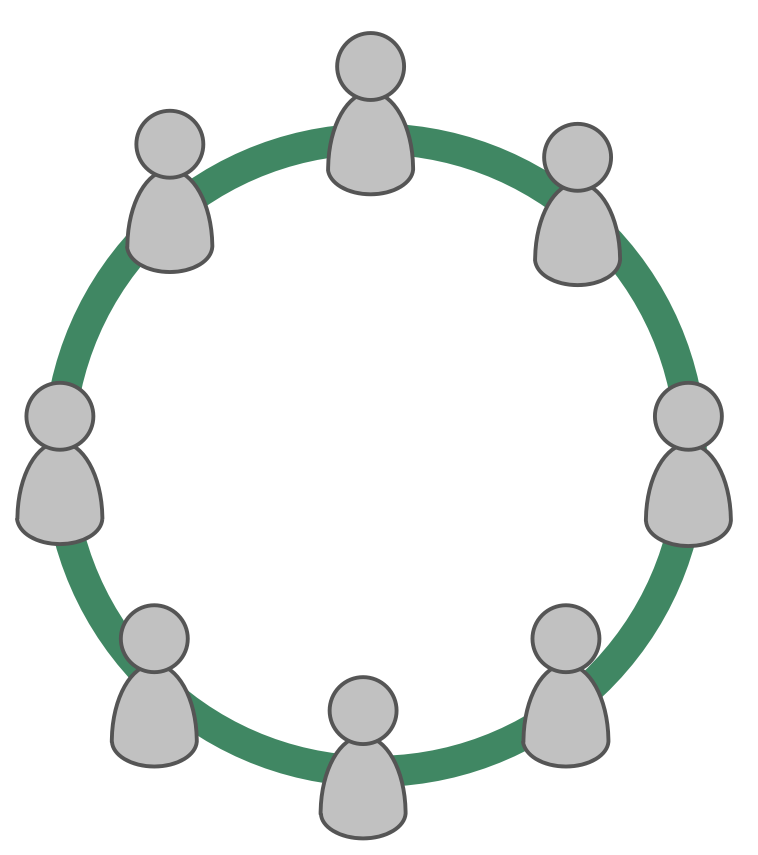
\includegraphics[width=\linewidth]{circulo.png}
	\caption{Todos/as los/as miembros/as de una comisión son igualmente responsables de las decisiones y actividades en su dominio.}
	\label{fig:circulo}
\end{marginfigure}

Las comisiones son responsables de su propio desarrollo y actúan como equipos de trabajo y puntos de toma de decisiones. Por ejemplo, la comisión de comunicaciones podría reunirse semanalmente por Hangouts para tomar decisiones \textbf{exclusivamente relevantes} a su área, y de topar con otros comisiones se elevaría esa decisión hacia la comisión de operaciones.

Una comisión debe definir en sus reuniones los \textbf{roles} que cada miembro va a tomar. Al ser todos los miembros equivalentes, no existen "puestos", sino roles que los facultan de ejecutar ciertas tareas, por ejemplo:
\begin{displayquote}
	Agustín Covarrubias se encarga de el manejo de Twitter, con tal de asegurar visibilidad a las actividades de la Asamblea. No puede publicar posts de contenido político sin aprobación de la comisión de comunicaciones. Este rol debe renovarse en dos semanas.
\end{displayquote}

Esto establece un marco claro para las atribuciones de cada persona, dando autonomía a cada persona a tomar las acciones necesarias para ejecutar su rol dentro de las restricciones puestas.

El método de toma de decisiones durante las reuniones es el \textbf{consenso} (el mismo mecanismo utilizado en Wikipedia y en la COP21), por el cual las propuestas o mociones se vuelven acuerdos cuando son consideradas \textit{lo suficientemente buenas por el momento, y suficientemente seguras para seguir
siendo evaluadas} por todos/as los/as integrantes. 

Esto no significa que estén 100\% de acuerdo, sino que consideran la moción lo suficientemente buena como para trabajar con ella. Si una objeción se determina difícil de resolver, se puede a través del mismo consenso acordar otro mecanismo de toma de decisiones (como una votación), pero la prioridad es resolver el conflicto intentando amendar la propuesta de forma iterativa. (fig. 2)
\begin{marginfigure}[-400px]
	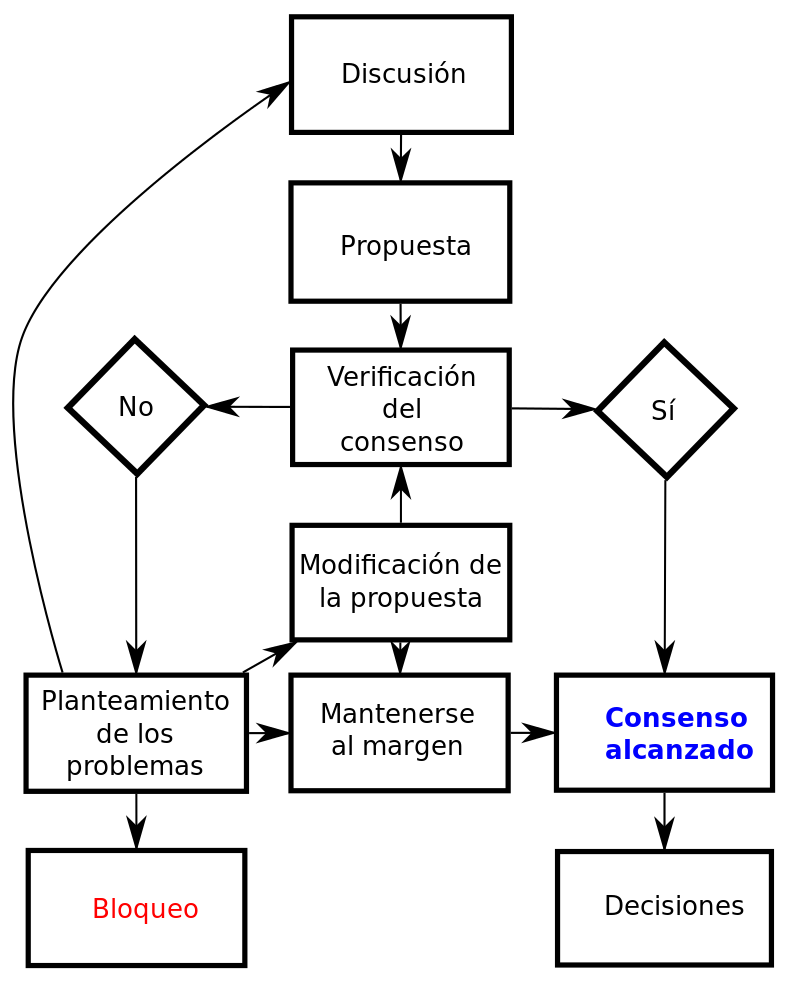
\includegraphics[width=\linewidth]{consenso.png}
	\caption{Diagrama de flujo de una decisión por consenso.}
	\label{fig:consenso}
\end{marginfigure}

A través del mismo consenso, cada comisión elige una pareja (preferiblemente paritaria) de delegados, renovada reunión por medio, que participa en representación de su comisión en la \textbf{comisión de operaciones}, una comisión (fig. 3) mayor reuniendo a delegados de todas las comisiones, y que por tanto toma decisiones operacionales que afecten múltiples áreas o comisiones, al igual que mociones que requieren atención o retroalimentación de todos y todas, sin poder negar aquellas atribuciones de Gobernanza. Es importante aclarar que los delegados no tienen ninguna autoridad interna por sobre los otros integrantes de su comisión, sino que buscan llevar y representar el cuerpo de acuerdos propio en la comisión de operaciones.

\begin{marginfigure}[-200px]
	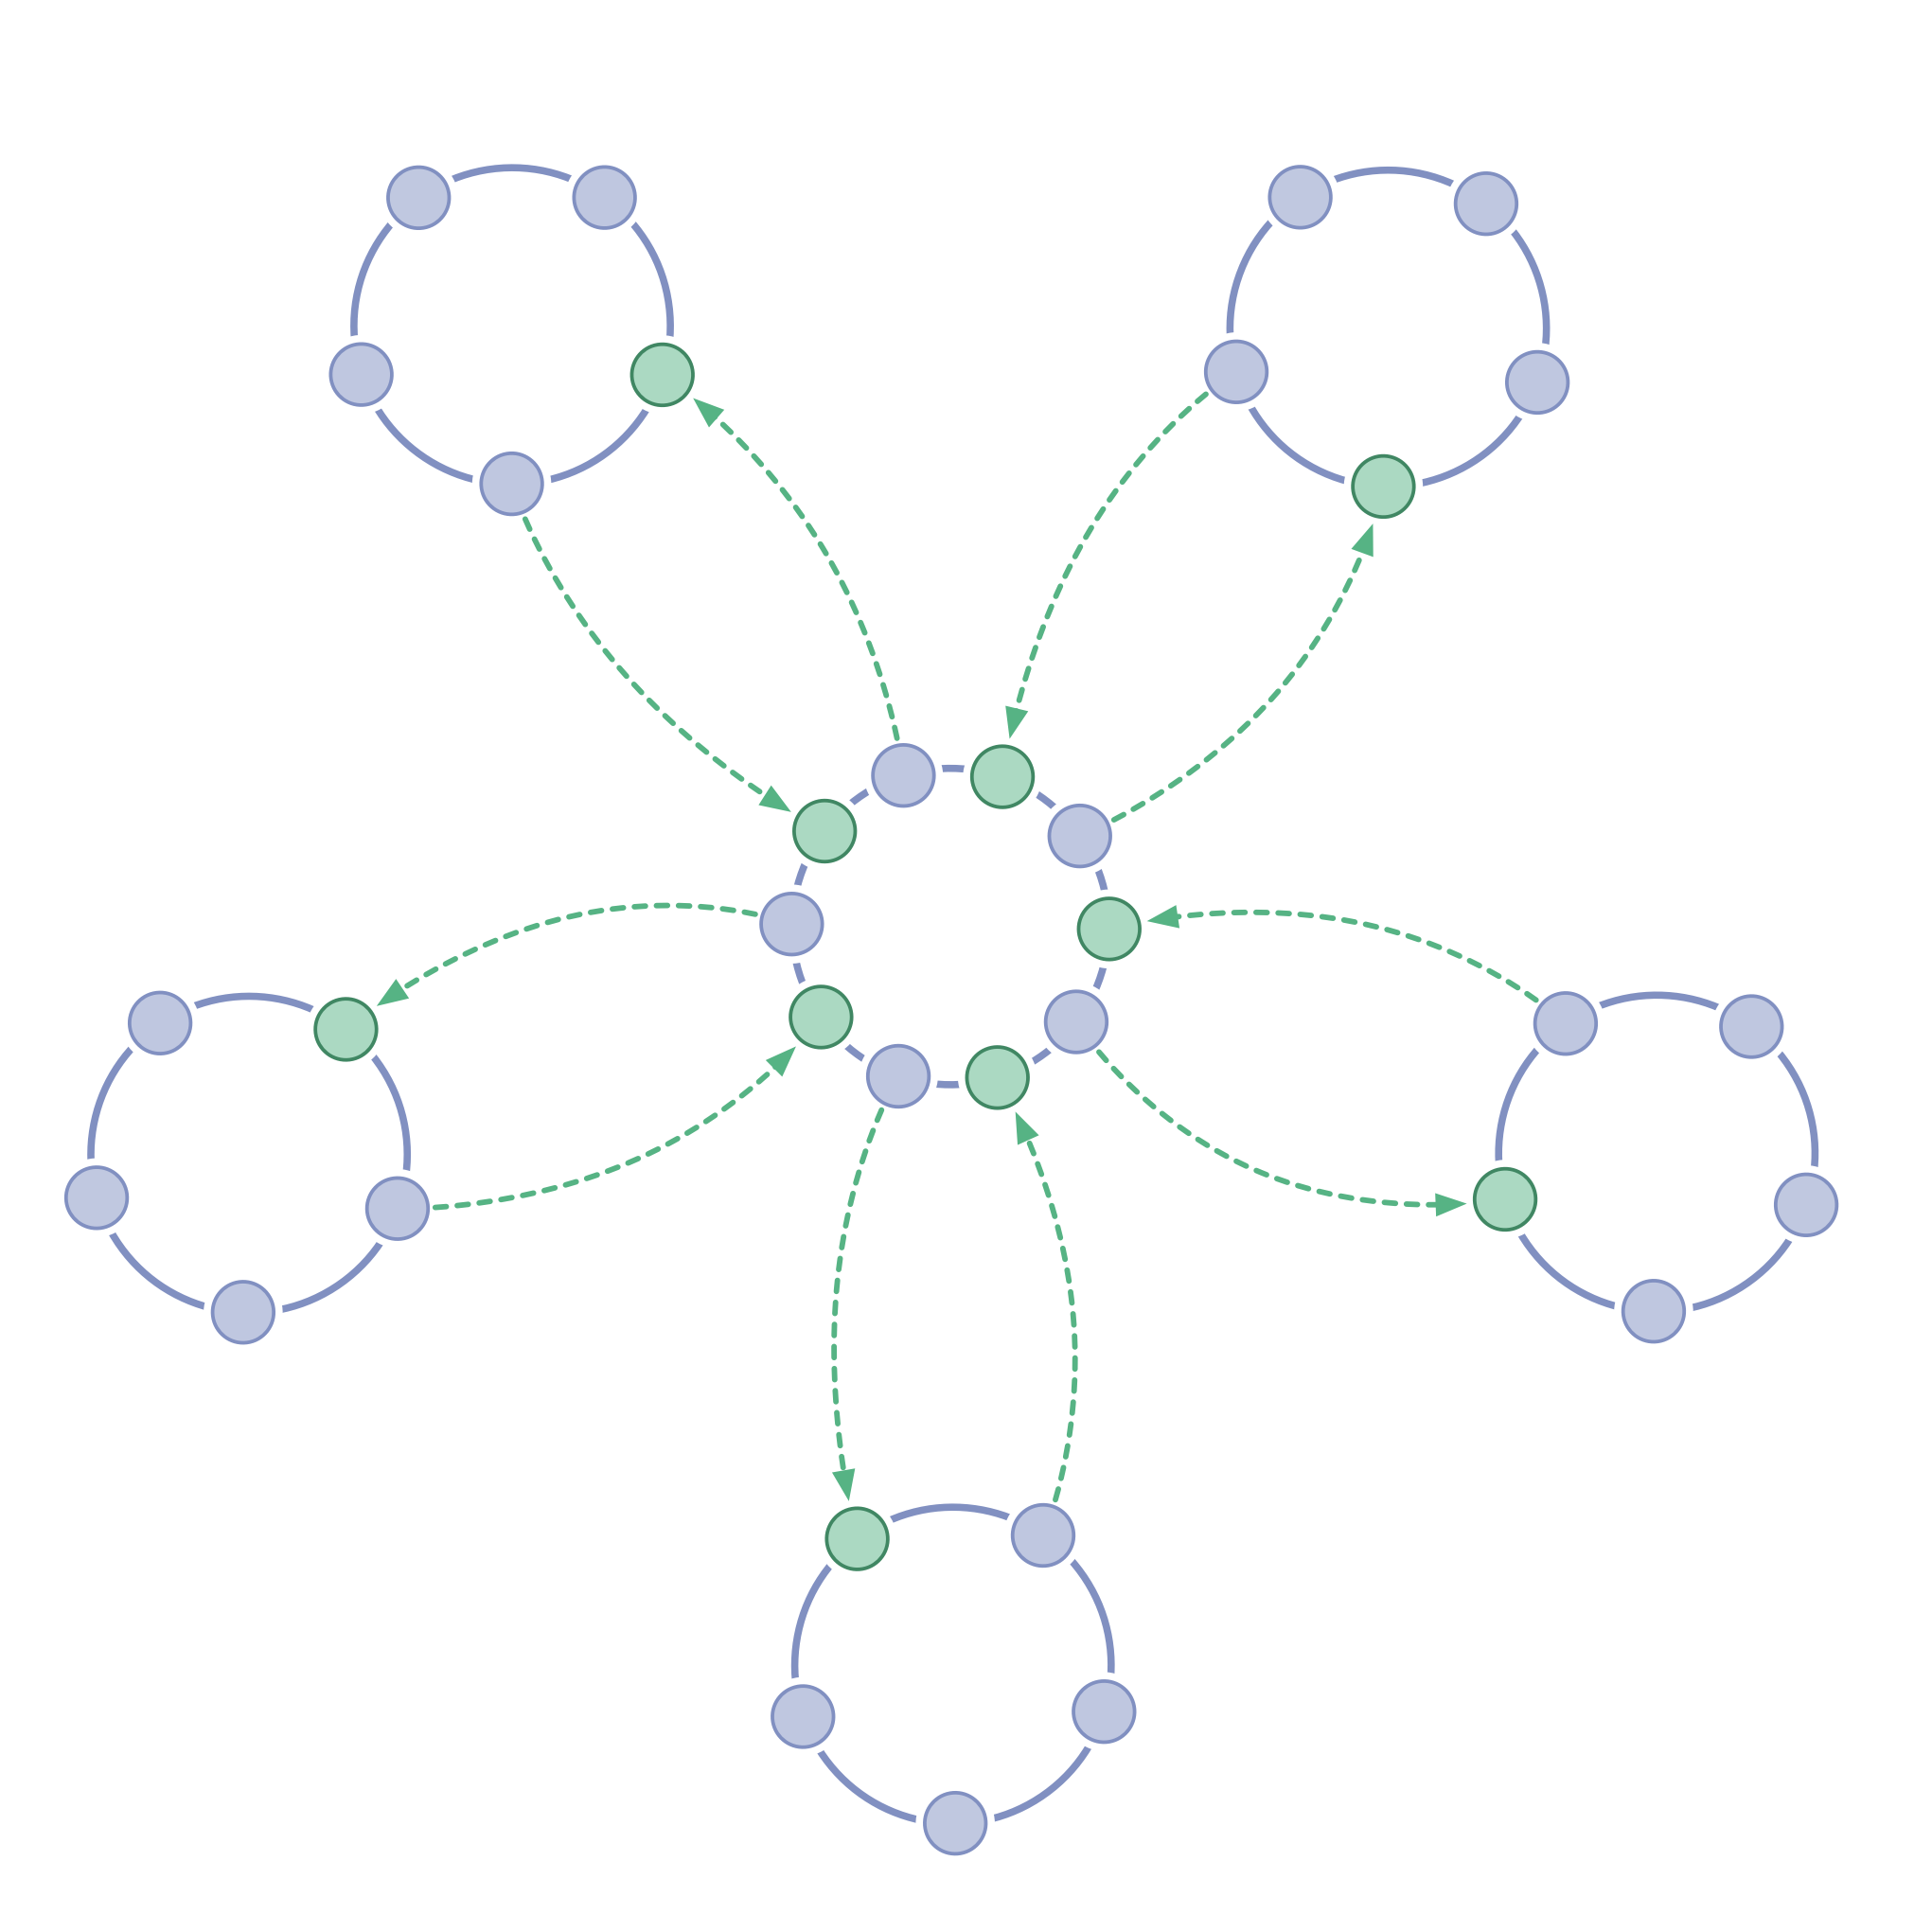
\includegraphics[width=\linewidth]{jerarquia.png}
	\caption{Cada comisión reúne dos delegados en una comisión mayor, llamada \textbf{comisión de operaciones.}}
	\label{fig:jerarquia}
\end{marginfigure}


\nobibliography{biblio}

\bibliographystyle{apa}

%----------------------------------------------------------------------------------------

\end{document}
